\documentclass{amsart}

\usepackage{tikz}
\usepackage{amsmath}
\usetikzlibrary{fit,arrows,calc,positioning}

\definecolor{heavyorange}{HTML}{FF7600}
\definecolor{almostblack}{HTML}{1a0f00}
\definecolor{lightorange}{HTML}{ffebcc}
\definecolor{lightgrey}{HTML}{f6f6f6}
\begin{document}
 
\begin{center}	
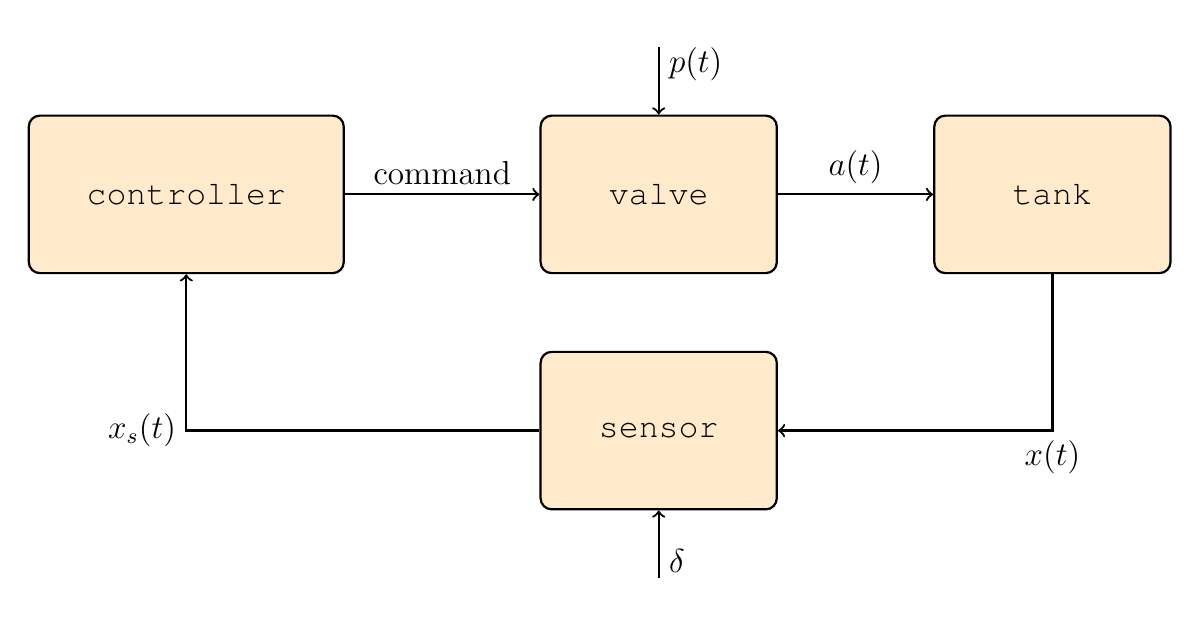
\begin{tikzpicture}
	 \begin{scope}[thick,font=\small]
		\draw (6,2) node[](p) {};	 
		\draw (6,-5) node[](delta) {};	
	        
		\draw (0,0) node[draw,rounded corners, minimum height=2cm, minimum width=4cm, fill=lightorange](controller) 
					{{\fontfamily{pcr}\selectfont \large controller}};
					
		\draw (6,0) node[draw,rounded corners, minimum height=2cm, minimum width=3cm, fill=lightorange](valve) 
					{{\fontfamily{pcr}\selectfont \large valve}};
					
		\draw (11,0) node[draw,rounded corners, minimum height=2cm, minimum width=3cm, fill=lightorange](tank) 
					{{\fontfamily{pcr}\selectfont \large tank}};
					
		\draw (6,-3) node[draw,rounded corners, minimum height=2cm, minimum width=3cm, fill=lightorange](sensor) 
					{{\fontfamily{pcr}\selectfont \large sensor}};
	
		\draw [->] (delta) -- (sensor) node[near start,right] 
					{\large $\delta$};									
		\draw [->] (p) -- (valve) node[near start,right] 
					{\large $p(t)$};					
		\draw [->] (controller) -- (valve) node[midway,above] 
					{\large command};
		\draw [->] (valve) -- (tank) node[midway,above] 
					{\large $a(t)$};
		\draw [->] (tank) |- (sensor) node[midway,below] 
					{\large $x(t)$};
		\draw [->] (sensor) -| (controller) node[midway,left] 
					{\large $x_s(t)$};
	 \end{scope}
\end{tikzpicture}
\end{center}

	
\end{document}